
\documentclass[a4paper,11pt]{article}
\usepackage[a4paper, margin=8em]{geometry}

% usa i pacchetti per la scrittura in italiano
\usepackage[french,italian]{babel}
\usepackage[T1]{fontenc}
\usepackage[utf8]{inputenc}
\frenchspacing 

% usa i pacchetti per la formattazione matematica
\usepackage{amsmath, amssymb, amsthm, amsfonts}

% usa altri pacchetti
\usepackage{gensymb}
\usepackage{hyperref}
\usepackage{standalone}

% imposta il titolo
\title{Appunti Elettronica Digitale}
\author{Luca Seggiani}
\date{2026}

% imposta lo stile
% usa helvetica
\usepackage[scaled]{helvet}
% usa palatino
\usepackage{palatino}
% usa un font monospazio guardabile
\usepackage{lmodern}

\renewcommand{\rmdefault}{ppl}
\renewcommand{\sfdefault}{phv}
\renewcommand{\ttdefault}{lmtt}

% disponi il titolo
\makeatletter
\renewcommand{\maketitle} {
	\begin{center} 
		\begin{minipage}[t]{.8\textwidth}
			\textsf{\huge\bfseries \@title} 
		\end{minipage}%
		\begin{minipage}[t]{.2\textwidth}
			\raggedleft \vspace{-1.65em}
			\textsf{\small \@author} \vfill
			\textsf{\small \@date}
		\end{minipage}
		\par
	\end{center}

	\thispagestyle{empty}
	\pagestyle{fancy}
}
\makeatother

% disponi teoremi
\usepackage{tcolorbox}
\newtcolorbox[auto counter, number within=section]{theorem}[2][]{%
	colback=blue!10, 
	colframe=blue!40!black, 
	sharp corners=northwest,
	fonttitle=\sffamily\bfseries, 
	title=~\thetcbcounter: #2, 
	#1
}

% disponi definizioni
\newtcolorbox[auto counter, number within=section]{definition}[2][]{%
	colback=red!10,
	colframe=red!40!black,
	sharp corners=northwest,
	fonttitle=\sffamily\bfseries,
	title=~\thetcbcounter: #2,
	#1
}

% U.D.M
\newcommand{\amp}{\ensuremath{\mathrm{A}}}
\newcommand{\volt}{\ensuremath{\mathrm{V}}}
\newcommand{\meter}{\ensuremath{\mathrm{m}}}
\newcommand{\second}{\ensuremath{\mathrm{s}}}
\newcommand{\farad}{\ensuremath{\mathrm{F}}}
\newcommand{\henry}{\ensuremath{\mathrm{H}}}
\newcommand{\siemens}{\ensuremath{\mathrm{S}}}

% circuiti
\usepackage{circuitikz}
\usetikzlibrary{babel}

% disegni
\usepackage{pgfplots}
\pgfplotsset{width=10cm,compat=1.9}

% disponi codice
\usepackage{listings}
\usepackage[table]{xcolor}

\definecolor{codegreen}{rgb}{0,0.6,0}
\definecolor{codegray}{rgb}{0.5,0.5,0.5}
\definecolor{codepurple}{rgb}{0.58,0,0.82}
\definecolor{backcolour}{rgb}{0.95,0.95,0.92}

\lstdefinestyle{codestyle}{
		backgroundcolor=\color{black!5}, 
		commentstyle=\color{codegreen},
		keywordstyle=\bfseries\color{magenta},
		numberstyle=\sffamily\tiny\color{black!60},
		stringstyle=\color{green!50!black},
		basicstyle=\ttfamily\footnotesize,
		breakatwhitespace=false,         
		breaklines=true,                 
		captionpos=b,                    
		keepspaces=true,                 
		numbers=left,                    
		numbersep=5pt,                  
		showspaces=false,                
		showstringspaces=false,
		showtabs=false,                  
		tabsize=2
}

\lstdefinestyle{shellstyle}{
		backgroundcolor=\color{black!5}, 
		basicstyle=\ttfamily\footnotesize\color{black}, 
		commentstyle=\color{black}, 
		keywordstyle=\color{black},
		numberstyle=\color{black!5},
		stringstyle=\color{black}, 
		showspaces=false,
		showstringspaces=false, 
		showtabs=false, 
		tabsize=2, 
		numbers=none, 
		breaklines=true
}

\lstdefinelanguage{javascript}{
	keywords={typeof, new, true, false, catch, function, return, null, catch, switch, var, if, in, while, do, else, case, break},
	keywordstyle=\color{blue}\bfseries,
	ndkeywords={class, export, boolean, throw, implements, import, this},
	ndkeywordstyle=\color{darkgray}\bfseries,
	identifierstyle=\color{black},
	sensitive=false,
	comment=[l]{//},
	morecomment=[s]{/*}{*/},
	commentstyle=\color{purple}\ttfamily,
	stringstyle=\color{red}\ttfamily,
	morestring=[b]',
	morestring=[b]"
}

% disponi sezioni
\usepackage{titlesec}

\titleformat{\section}
	{\sffamily\Large\bfseries} 
	{\thesection}{1em}{} 
\titleformat{\subsection}
	{\sffamily\large\bfseries}   
	{\thesubsection}{1em}{} 
\titleformat{\subsubsection}
	{\sffamily\normalsize\bfseries} 
	{\thesubsubsection}{1em}{}

% disponi alberi
\usepackage{forest}

\forestset{
	rectstyle/.style={
		for tree={rectangle,draw,font=\large\sffamily}
	},
	roundstyle/.style={
		for tree={circle,draw,font=\large}
	}
}

% disponi algoritmi
\usepackage{algorithm}
\usepackage{algorithmic}
\makeatletter
\renewcommand{\ALG@name}{Algoritmo}
\makeatother

% disponi numeri di pagina
\usepackage{fancyhdr}
\fancyhf{} 
\fancyfoot[L]{\sffamily{\thepage}}

\makeatletter
\fancyhead[L]{\raisebox{1ex}[0pt][0pt]{\sffamily{\@title \ \@date}}} 
\fancyhead[R]{\raisebox{1ex}[0pt][0pt]{\sffamily{\@author}}}
\makeatother

\begin{document}
% sezione (data)
\section{Lezione del 06-03-26}

% stili pagina
\thispagestyle{empty}
\pagestyle{fancy}

% testo
Alla fine della lezione 2 abbiamo trattato il \textit{silicio intrinseco}. In particolare, avevamo definito i fenomeni di:
\begin{itemize}
	\item \textbf{Generazione termica}: sottoposto a calore, il silicio assorbe energia che rompe i legami portando alla formazione di coppie \textit{elettrone}/\textit{lacuna} ($e$/$h$, da $h$ di \textit{hole}, o come abbiamo detto in altri contesti coppie $(-1 e, +1 e)$);
	\item \textbf{Ricombinazione termica}: in tandem alla generazione termica, si ha un fenomeno di ricombinazione degli elettroni nei legami del silicio, che annichilisce le coppie elettrone/lacuna. 
\end{itemize}

A conti fatti si aveva che il numero di portatori di carica (elettroni o lacune) disponibili alla conduzione era:
$$
n = p = n_i = \text{generazione termica} + \text{ricombinazione termica}
$$
in condizioni di equilibrio con le frequenze di generazione termica $G$ e di ricombinazione termica $R$:
$$
G = R
$$
e la conduttività era quindi:
$$
\sigma = n \mu_n e + p \mu_p e
$$
che si otteneva a partire dell'espressione della velocità di deriva in funzione della mobilità elettronica $\mu_n$ o di lacuna $\mu_p$, e dalla legge microscopica di Ohm (legge 2.1).

\par\smallskip

\noindent
\textbf{\textsf{Stima della conduttanza intrinseca}}

\noindent
Ricordiamo che a $300 \, \mathrm{K}$ gradi Kelvin, il numero di elettroni liberi nel silicio è circa $10^{10} \, \mathrm{cm}^{-3}$. Prendendo i valori di mobilità elettronica e di lacuna del silicio:
\begin{table}[H]
	\center \rowcolors{2}{white}{black!10}
	\begin{tabular} { c | c | c  }
		\bfseries Quantità & \bfseries Simbolo & \bfseries Valore \\
		\hline 
		Mobilità elettronica & $\mu_n$ & $1350  \, \frac{\mathrm{cm}^2}{\mathrm{V} \cdot \mathrm{s}}$ \\
		Mobilità delle lacune & $\mu_p$ & $480  \, \frac{\mathrm{cm}^2}{\mathrm{V} \cdot \mathrm{s}}$
	\end{tabular}
\end{table}
e svolgendo i calcoli si ha:
$$
\sigma = 10^{10} \cdot 1350 \cdot (1.6 \times 10^{-19}) + 10^{10} \cdot 480 \cdot (1.6 \times 10^{-19}) = 3 \times 10^{-6} \, \Omega \cdot \mathrm{cm}^{-1}
$$
che di base rende il silicio intrinseco un cattivo conduttore.

\subsection{Drogaggio del silicio}
Possiamo quindi approfondire il concetto del \textbf{drogaggio} del silicio introdotto in 1.2.2. Di base, la legge che ci risulterà utile per valutare i portatori di carica di un conduttore non intrinseco sarà quella che lega il numero di portatori di carica negativi e positivi (elettroni e lacune) nel semiconduttore estrinseco alla concentrazione di elettroni (o ugualmente, lacune) nel corrispondente intrinseco:
\begin{definition}{Legge azione di massa}
Il nunmero di portatori di carica negativi $n$ e positivi $p$ in un semiconduttore rispetta la relazione:	
$$
n \cdot p = n_i^2
$$
dove $n_i$ è la concentrazione di elettroni liberi nel silicio intrinseco.
\end{definition}

Questo è in opposizione alla legge che valeva nei semiconduttori intrinsechi, dove parlare di $p$ o $n$ era indifferente in quanto:
$$
n = p = n_i
$$

Quello che succede è che si può portare il silicio a formare legami con altri elementi, in particolare:
\begin{itemize}
	\item Con quelli del quinto gruppo della tavola periodica (fra cui il fosforo, simbolo $[\mathrm{P}])$, e l'arsenico, simbolo $[\mathrm{As}]$), che chiamiamo drogaggio di tipo \textbf{n} (perché come vedremo aumenta il numero di portatori negativi, cioè elettroni);
	\item Con quelli del terzo gruppo della tavola periodica (fra cui il boro, simbolo $[\mathrm{B}]$), che chiamiamo drogaggio di tipo \textbf{p} (perché come vedremo, in maniera duale al precedente, aumenta il numero di portatori positivi, cioè lacune).
\end{itemize}

Togliamoci anche la curiosità di come si svolge il processo di drogaggio del silicio dal punto di vista tecnico: 
\begin{itemize}
	\item 
Abbiamo che un primo metodo sfrutta il processo della \textit{diffusione} (che vedremo nel dettaglio in 4.2 riguardo alla corrente di diffusione, ma qui agisce in un contesto chimico diverso). Questo è il processo più diffuso in laboratorio. In particolare, si stende un \textit{film} di materiale drogante sul substrato di silicio, che viene poi riscaldato e quindi (appunto per \textit{diffusione}) va a legare col substrato.
	\item
Su scala industriale, invece, si mira ad usare un processo di \textit{impiantazione ionica}. Questo metodo consiste nel bombardare il substrato con ioni di materiale dopante, forzando quindi in qualche modo i legami di atomi donatori o accettori. Notiam oche questo processo rovina il materiale, per cui in seguito si necessita di un processo di \textit{annealing} termico che permetta la ricostruzione della struttura cristallina.
\end{itemize}

\subsubsection{Drogaggio di tipo N}
Vediamo cosa accade nel drogaggio con atomi del quinto gruppo. Ad esempio, prendiamo in considerazione il fosforo, che ha configurazione elettronica $[\mathrm{Ne}] 3s^2 3p^3$, e quindi 5 elettroni liberi nello strato di valenza. 

Ciò che andiamo a fare è quindi sostituire una certa percentuale degli atomi di silicio nel reticolo cristallino con atomi di fosforo. Questi mettono i loro 4 elettroni al servizio dei legami covalenti con i 4 atomi di silicio adiacenti. Il quinto elettrone resta molto debolmente legato al nucleo di fosforo, per cui la maggior parte degli atomi ionizzano a temperatura ambiente (finora abbiamo parlato di $T = 300 \, \mathrm{K}$). 

Chiamiamo $N_D$ la concentrazione di tali atomi, detti \textit{donatori}. Solitamente possiamo dire:
$$
N_D = [10^{14}, 10^{21}] \, \mathrm{cm}^{-3}
$$
dove notiamo che se $N_D = 10^{21}$ la concentrazione al centimetro cubo è quasi uguale alla mole, cioè abbiamo quasi interamente sostituito gli atomi di silicio. 

Abbiamo quindi che in condizione di regime del silicio drogato con un elemento del quinto gruppo, i processi di \textit{generazione} e \textit{ricombinazione} termica avvengono comunque, ma parte integrante degli elettroni liberi vengono forniti dagli atomi donatori. In particolare, vale la stima:
$$
n \approx N_D \implies p \approx \frac{n_i^2}{n} = \frac{n_i^2}{N_D}
$$
visto che come abbiamo detto la maggior parte degli atomi donatori $N_D$ ionizza.

Diciamo che gli $n$ sono conduttori \textbf{maggioritari} (gli elettroni, crescono all'aumentare del drogaggio), mentre gli $p$ sono conduttori \textbf{minoritari} (le lacune, diminuiscono all'aumentare del drogaggio).

\par\smallskip

\noindent
\textbf{\textsf{Stima della conduttanza con drogaggio di tipo N}}

\noindent
Prendiamo un valore $N_D = 10^{15} \, \mathrm{cm}^{-3}$ e calcoliamo nuovamente il valore della conduttanza. Notiamo che a seguito del processo di drogaggio i valori di mobilità elettronica e di lacuna cambiano, come vedremo in 4.1.3:
\begin{table}[H]
	\center \rowcolors{2}{white}{black!10}
	\begin{tabular} { c | c | c  }
		\bfseries Quantità & \bfseries Simbolo & \bfseries Valore \\
		\hline 
		Mobilità elettronica & $\mu_n$ & $1320  \, \frac{\mathrm{cm}^2}{\mathrm{V} \cdot \mathrm{s}}$ \\
		Mobilità delle lacune & $\mu_p$ & $460  \, \frac{\mathrm{cm}^2}{\mathrm{V} \cdot \mathrm{s}}$
	\end{tabular}
\end{table}

Avremo quindi bisogno di ricavare $n$ e $p$ con le relazioni appena trovate:
$$
n = N_D = 10^{15} \, \mathrm{cm}^{-3}, \quad p = \frac{(10^{10})^2}{10^{15}} = 10^5 \, \mathrm{cm}^{-3}
$$

Si ha quindi che la conduttanza, riprendendo la formula dello scorso esempio, sarà:
$$
\sigma = 10^{15} \cdot 1320 \cdot (1.6 \times 10^{-19}) + 10^{5} \cdot 460 \cdot (1.6 \times 10^{-19}) = 0.211 \, \Omega \cdot \mathrm{cm}^{-1}
$$
cioè introducendo un doping del:
$$
\frac{10^{15}}{10^{22}} \sim 10^{-7}
$$
ovvero variando un atomo di silicio su $10^{7}$ con un atomo del quinto gruppo, siamo riusciti ad ottenere un aumento della conduttanza di ben 5 ordini di grandezza.

\subsubsection{Drogaggio di tipo P}
Vediamo quindi cosa accade con drogaggio con un elemento del terzo gruppo. In questo caso prendiamo l'esempio del boro, che ha configurazione elettronica $[\mathrm{He}] 2s^2 2p^1$, e quindi 3 elettroni liberi nello strato di valenza. 

Se procediamo col drogaggio al boro, quindi sostituendo alcuni atomi di silicio con atomi di boro, ciò che accade è che i 3 elettroni di valenza vanno a formare legami covalenti nel reticolo cristallino del silicio. Il quarto legame non può essere formato (in quanto quell'elettrone non c'è), per cui si forma naturalmente una lacuna elettronica. Anzi, abbiamo che gli atomi di silicio stessi ionizzano, cedendo elettroni all'atomo di boro (che diventa quindi ione negativo).

In questo caso abbiamo quindi la densità $N_A$ di atomi, detti \textit{accettori}. Solitamente possiamo dire:
$$
N_A = [10^{14}, 10^{21}] \, \mathrm{cm}^{-3}
$$

Abbiamo quindi che in condizione di regime del silicio drogato con un elemento del terzo gruppo, i conduttori maggioritari sono le lacune (in maniera totalmente duale al drogaggio del tipo N). In particolare, vale la stima:
$$
p \approx N_A \implies n \approx \frac{n_i^2}{p} = \frac{n_i^2}{N_A}
$$
data dal fatto che quasi ogni atomo di boro introdotto ionizza.

Notiamo che stavolta gli $p$ sono conduttori \textbf{maggioritari} (le lacune, crescono all'aumentare del drogaggio), mentre gli $n$ sono conduttori \textbf{minoritari} (gli elettroni, diminuiscono all'aumentare del drogaggio).

\par\smallskip

\noindent
\textbf{\textsf{Stima della conduttanza con drogaggio di tipo P}}

\noindent
Prendiamo un valore $N_A = 10^{15} \, \mathrm{cm}^{-3}$ e calcoliamo nuovamente il valore della conduttanza. Anche qui, a seguito del processo di drogaggio i valori di mobilità elettronica e di lacuna cambiano:
\begin{table}[H]
	\center \rowcolors{2}{white}{black!10}
	\begin{tabular} { c | c | c  }
		\bfseries Quantità & \bfseries Simbolo & \bfseries Valore \\
		\hline 
		Mobilità elettronica & $\mu_n$ & $1350  \, \frac{\mathrm{cm}^2}{\mathrm{V} \cdot \mathrm{s}}$ \\
		Mobilità delle lacune & $\mu_p$ & $450  \, \frac{\mathrm{cm}^2}{\mathrm{V} \cdot \mathrm{s}}$
	\end{tabular}
\end{table}

Avremo quindi bisogno di ricavare $n$ e $p$ con le relazioni appena trovate:
$$
n = \frac{(10^{10})^2}{10^{15}} = 10^5 \, \mathrm{cm}^{-3}, \quad p = N_A = 10^{15} \, \mathrm{cm}^{-3}
$$

Si ha quindi che la conduttanza, riprendendo la formula dello scorso esempio, sarà:
$$
\sigma = 10^{5} \cdot 1350 \cdot (1.6 \times 10^{-19}) + 10^{15} \cdot 450 \cdot (1.6 \times 10^{-19}) = 0.072 \, \Omega \cdot \mathrm{cm}^{-1}
$$
cioè introducendo un doping del:
$$
\frac{10^{15}}{10^{22}} \sim 10^{-7}
$$
ovvero variando un atomo di silicio su $10^{7}$ con un atomo del terzo gruppo, siamo riusciti ad ottenere un aumento della conduttanza di 4 ordini di grandezza. Questo non è buono quanto quello che eravamo riusciti ad ottenere col drogaggio al fosforo (visto che la mobilità di lacuna è molto minore della mobilità elettronica), ma è comunque valido.

\par\smallskip

\noindent
\textbf{\textsf{Legami alla teoria delle bande}}

\noindent
In 2.1.3, parlando della corrente di deriva nei semiconduttori (intrinseci, prima del drogaggio, che abbiamo introdotto adesso) avevamo accennato alla \textit{teoria delle bande}. L'idea fondamentale di questa era di considerare il reticolo cristallino di un semiconduttore, con elettroni e lacune libere, come un sistema di particelle dotate di stati energetici $N$. In particolare avevamo detto che il numero di portatori liberi in un semiconduttore era legato alla statistica di Maxwell-Boltzmann, usata per stimare la densità di conduttori sulla banda di conduzione (legge 2.2). Abbiamo che variando la composizione del reticolo (attraverso il drogaggio), si vanno a variare le caratteristiche di tali particelle e quindi le statistiche (seppur leggermente).
\begin{center}
	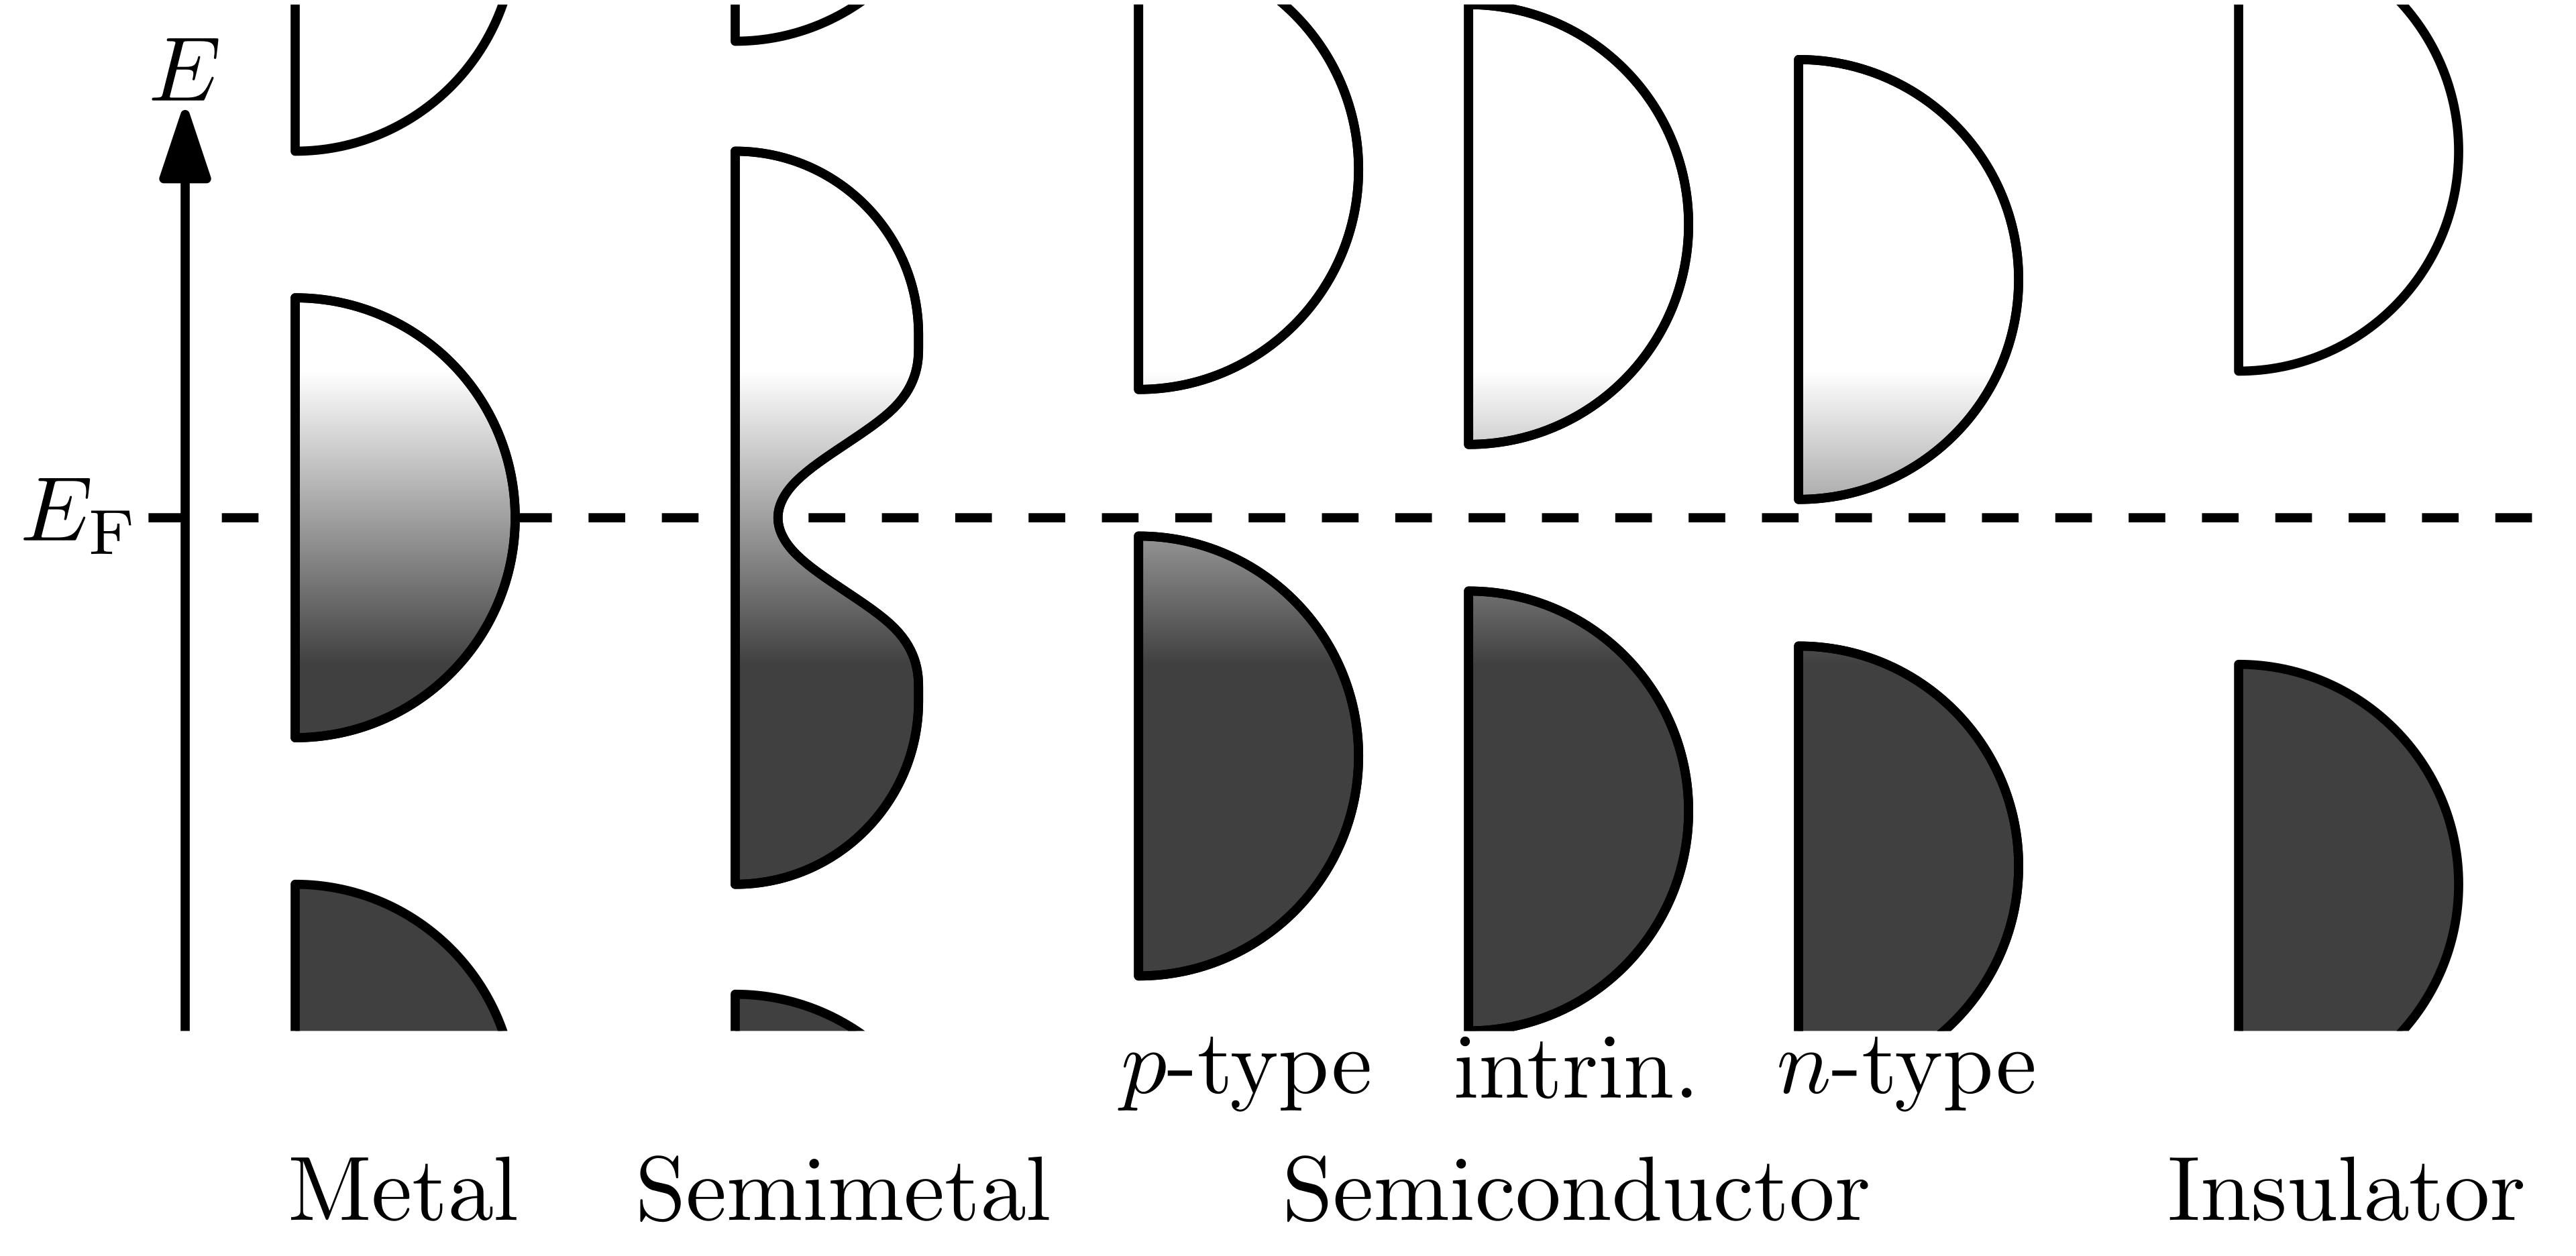
\includegraphics[scale=0.08]{../figures/band_doping.png}
\end{center}
Vediamo adesso che l'effetto del drogaggio a livello di teoria delle bande è che il livello di Fermi (che avevamo visto nei semiconduttori si andava a trovare all'interno dell'intervallo energetico $E_G$ fra la banda di valenza e la banda di conduzione) si sposta verso l'alto o verso il basso:
\begin{itemize}
	\item Nel caso di drogaggio di tipo \textbf{p}, il livello di Fermi si sposta in basso: questo significa che gli elettroni diventano più "difficili" da eccitare, e si ha maggioranza di lacune;
	\item Nel caso di drogaggio di tipo \textbf{n}, il livello di Fermi si sposta in alto. Questo significa che si gli elettroni diventano più "facili" da eccitare, e si ha maggioranza elettronica.
\end{itemize}

\par\smallskip

\noindent
\textbf{\textsf{Drogaggi multipli}}

\noindent
Notiamo che si può effettuare un processo di drogaggio di tipo sia N che P. In particolare, se su un substrato di tipo N si fa un forte drogaggio di tipo P, effettivamente il tipo di drogaggio viene invertito. Viceversa, se su un substrato di tipo P si fa un forte drogaggio di tipo N, nuovamente il drogaggio viene invertito.

Cioè, in sostanza, si può ottenere silicio estrinseco di tipo P, N, o silicio intrinseco, sulla base del tipo di drogaggio che viene fatto anche in più passate sul substrato.

\subsubsection{Stima delle mobilità}
Riprendiamo la formula per la conducibilità:
$$
\sigma = n \mu_n e + p \mu_p e = f(T)
$$

Qui ricordiamo che compaiono:
\begin{itemize}
	\item La \textit{mobilità elettronica} dei portatori di carica negativi, cioè gli elettroni;
	\item La \textit{mobilità di lacuna} dei portatori di carica positivi, cioè le lacune. Queste sarebbero legami che \textit{"saltano"} da un atomo all'altro, che però possiamo semplicemente considerare come elettroni \textit{"positivi"} che si spostano nel reticolo del semiconduttore.
\end{itemize}

Abbiamo che $\sigma$ stessa è dipendente dalla temperatura $T$ sulla base della variazione delle concentrazioni $n$ e $p$. Si scopre che anche $\mu_n$ e $\mu_p$ sono dipendenti da $T$, e in particolare:
\begin{itemize}
	\item $\mu_n$, $\mu_p$: diminuiscono all'aumentare di $T$ (in particolare sono propozionali a $T^{-\frac{3}{2}}$);
	\item $n$, $p$: qui dobbiamo considerare i vari casi di drogaggio o meno:
		\begin{itemize}
			\item Per quanto riguarda il silicio \textbf{intrinseco}, vale:
				$$
					n = p = n_i
				$$
				e quindi $n$, $p$ aumentano esponenzialmente come $n_i$ (rispettando la legge 2.4). Questo significa che in media $\sigma$ \textit{aumenta} con $T$ (in quanto le concentrazioni $n$, $p$ aumentano più di quanto diminuiscono le mobilità $\mu_n$, $\mu_p$);
			\item Nel caso del silicio drogato, la situazione cambia. Consideriamo prima il caso del drogaggio di tipo \textbf{N}. Valgono le stime riguardo alle concentrazioni:
				$$
				n \approx N_D, \quad p \approx \frac{n_i^2}{N_D}
				$$
				cioè $n$ resta costante sulla concentrazione di atomi donatori, mentre $p$ aumenta con $T$. Notiamo che aumenta \textit{poco}, in quanto di base $p$ rappresenta la concentrazione di conduttori \textit{minoritari} (le lacune). In questo caso, considerando anche la diminuzione di mobilità sulla base di $T$, si ha che complessivamente la conduttività \textit{diminuisce} con $T$.
			\item Vediamo quindi il drogaggio di tipo \textbf{B}. Valgono le stime riguardo alle concentrazioni:
				$$
				p \approx N_A, \quad n \approx \frac{n_i^2}{N_A}
				$$
				cioè $p$ resta costante sulla concentrazione di atomi accettori, mentre $n$ aumenta con $T$. Notiamo che aumenta \textit{poco}, in quanto di base $n$ rappresenta la concentrazione di conduttori \textit{minoritari} (gli elettroni). Come prima, considerando anche la diminuzione di mobilità sulla base di $T$, si ha che anche qui la conduttività \textit{diminuisce} con $T$. 
		\end{itemize}
\end{itemize}

Notiamo che quanto detto sul silicio drogato vale per temperature alte \textit{moderate}: a temperature $T$ abbastanza alte si ha che il processo di generazione e ricombinazione termica (che ricordiamo era governato dalla statistica Maxwelliana a 2.3, esponenziale alla temperatura) supera la riduzione di mobilità. In questo nuovo regime, che diciamo regime \textit{intrinseco} del silicio drogato, si ha che la conduttività ricomincia a salire. 

\subsection{Corrente di diffusione}
Abbiamo quindi concluso la trattazione delle correnti di \textit{deriva} nei conduttori e nei semiconduttori. Esiste un altro fenomeno di conduzione, particolarmente osservabile nei semiconduttori, detto \textbf{diffusione}. Il fenomeno della diffusione porta alla formazione della \textit{corrente di diffusione}.

In generale, la diffusione è un meccanismo che avviene ogni volta che si ha un \textit{gradiente di concentrazione} di un dato portatore (di carica, un gas, ecc...). Per via dell'\textit{agitazione termica}, il sistema tende naturalmente ad uno stato di equilibrio dove la concentrazione è uguale in ogni punto dello spazio. Dinamicamente, questo significa che le zone di \textit{alta} concentrazione diffondono verso le zone di \textit{bassa} concentrazione.
Le leggi che descrivono questi fenomeni sono le leggi di \textit{Fick} sulle diffusioni di concentrazioni. Semplificando un po' si ha in sostanza:
\begin{definition}{Legge di Fick}
	Il flusso di una concentrazione $\phi$ è legato al suo gradiente come:
	$$
	\vec{J} = -D \nabla \phi
	$$
	dove $D$ è la \textit{costante di diffusione} di $\phi$.
\end{definition}

Un fenomeno di questo tipo avviene anche per gli elettroni e le lacune in un semiconduttore. Supponiamo di avere un corpo esteso sull'asse $x$, ed un certo gradiente di concentrazione degli elettroni $n$ che varia sulla base di $x$ (cioè va come una certa funzione $n(x)$). Diciamo che $n(x)$ ha un picco per $x = 0$, cioè ha una forma del tipo:
$$
n(x) = e^{-x}, \ {x \geq 0}
$$

In questo caso vicino a $x = 0$ si avrà una zona di alta generazione e ricombinazione termica. Questo porterà ad un fenomeno di diffusione che, appunto, diffonderà portatori di carica (elettroni) verso $x >> 0$. Notiamo che questo porta alla formazione di una corrente (in quanto ci sono cariche che si spostano), nella direzione opposta a quella di diffusione.
Ad esempio, se si ha una diffusione di elettroni $e$ verso \textit{destra}, si forma una densità di corrente $\vec{J}$ rivolta verso sinistra.

\par\smallskip

\noindent
\textbf{\textsf{Diffusione elettronica}}

\noindent
Cerchiamo di calcolare questa densità di corrente per i soli elettroni:
$$
\vec{J} = - (-e) D_n \left(\frac{\partial n}{\partial x} \right) \hat{i}_x = e D_n \frac{\partial n}{\partial x} \hat{i}_x 
$$
dove $D_n$ è la costante di diffusione vista nella legge di Fick, una quantità analoga alla \textit{mobilità} considerata per la corrente di deriva e dipendente dalla deriva data dal fenomeno di diffusione. Il segno meno alla derivata parziale, come abbiamo detto, è dato dal fatto che gli elettroni si spostano in direzione opposta alla corrente. Questa legge deriva direttamente dalla legge di Fick (4.2), dove $\frac{\partial n}{\partial x}$ non è altro che la versione bidimensionale del gradiente $\nabla \phi$ (in questo caso $\nabla n$).

\par\smallskip

\noindent
\textbf{\textsf{Diffusione di lacune}}

\noindent
Possiamo calcolare la corrente di diffusione anche considerando solo i portatori positivi (le lacune):
$$
\vec{J} = - e D_p \left(\frac{\partial n}{\partial x} \right) \hat{i}_x = - e D_p \frac{\partial n}{\partial x} \hat{i}_x 
$$
dove $D_p$ è la costante di diffusione di lacuna (per distinguerla dalla costante di diffusione elettronica $D_n$). Chiaramente, stavolta le cariche si prendono come positive.

\subsubsection{Stima delle costanti di diffusione}

Potremmo voler stimolare le costanti di diffusione, o almeno legarle a costanti che conosciamo (magari le mobilità elettroniche e di lacuna $\mu_n$, $\mu_p$). Per questo ci torna utile la seguente legge:
\begin{definition}{Legge di Einstein delle costanti di diffusione}
	Riguardo alle costanti di \textit{diffusione} e le \textit{mobilità} di semiconduttori, possiamo applicare la stima:
	$$
		\frac{D_n}{\mu_n} = \frac{D_p}{\mu_p} = \frac{k_B T}{e} = V_T 
	$$
\end{definition}
dove $K_B$ è la costante di \textit{Boltzmann} già vista nella legge 2.1, e $V_T$ è la cosiddetta \textit{tensione termica}, che a $300 K$ vale circa $V_T = 26 \, m V$. Non diamo l'origine di questa formula (deriva dagli studi di Einstein sul \textit{moto browniano}), ma vediamo che la proporzione:
$$
D_n : \mu_n = D_p : \mu_p
$$
sembra ragionevole, in quanto particelle più mobili saranno più disposte a diffondere.

\subsubsection{Combinazione di correnti di drift e di diffusione}
Completiamo quindi il nostro modello combinando le densità di corrente di \textit{drift} e di \textit{diffusione}, che chiamiamo rispettivamente $\vec{J}_{\text{Drift}}$ e $\vec{J}_{\text{Diffusione}}$.

\begin{itemize}
	\item Prendendo le sole cariche elettroniche, cioè i portatori negativi, si ha:
$$
\vec{J}_N = \vec{J}_{N, \text{Drift}} + \vec{J}_{N, \text{Diffusione}} = n e \mu_n \vec{E} + e D_n \frac{\partial n}{\partial x} \hat{i}_x
$$
ricavato dalla legge microscopica di Ohm al primo termine (legge 2.3), e la legge di Fick (4.2) al secondo.
	\item Prendendo le sole cariche positive (le lacune elettroniche), cioè i portatori positivi, si ha:
$$
\vec{J}_P = \vec{J}_{P, \text{Drift}} + \vec{J}_{P, \text{Diffusione}} = p e \mu_p \vec{E} - e D_P \frac{\partial n}{\partial x} \hat{i}_x
$$
in maniera totalmente analoga alla scorsa derivazione.
\end{itemize}

La densità di corrente complessiva sarà quindi quella ottenuta combinando i nostri modelli:
$$
\vec{J}_N + \vec{J}_P = \vec{J}_{N, \text{Drift}} + \vec{J}_{N, \text{Diffusione}} + \vec{J}_{P, \text{Drift}} + \vec{J}_{P, \text{Diffusione}} = n e \mu_n \vec{E} + e D_n \frac{\partial n}{\partial x} \hat{i}_x + p e \mu_p \vec{E} - e D_P \frac{\partial n}{\partial x} \hat{i}_x 
$$

Tutte queste caratteristihe, quindi (drift e diffusione) vanno tenute in considerazione per stimare in maniera corretta la densità di corrente, in particolare in un semiconduttore.

\end{document}
